\documentclass[12pt,a4paper,fleqn]{article}
\title{Progress Report}
\author{Syed Ahmad Raza}
\date{2018.01.10}
\usepackage{mathtools}
\usepackage{graphicx}
\usepackage{color}          % for color eps output
% \usepackage{afterpage}
\usepackage{float}          % to force a figure placement with [H] command
\usepackage{enumitem}
\usepackage{newtxtext}
\usepackage{newtxmath}
%\usepackage{layouts}       % for: \printinunitsof{in}\prntlen{\textwidth}

\begin{document}
\maketitle
%\tableofcontents
\pagebreak

\section{Solution of Navier-Stokes equations using\\
    Finite Volume Method for nonuniform grid}

\subsection{Discretization of the convective and diffusive terms}

\begin{figure}[H]
    \centering
    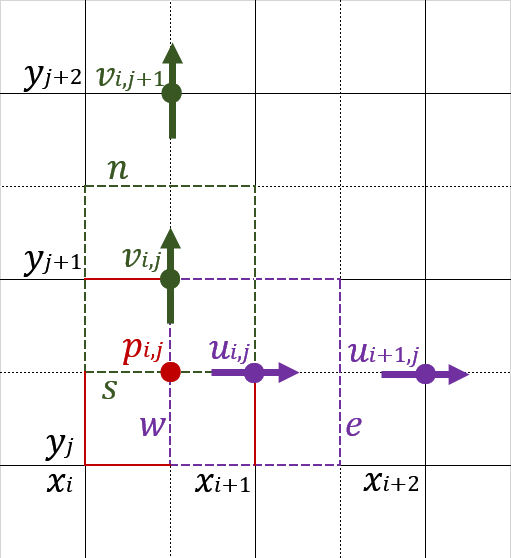
\includegraphics[width=0.5\textwidth]{staggered_grid.png}
    \caption{Visual representation of the staggered grid used for discretization in Finite Volume Method}
    \label{fig:staggered-grid}
\end{figure}

The convective and diffusive terms of Navier-Stokes equations can be discretized using the individual components. Using Chorin's projection method, the $u$-component equation can be written as
\begin{equation} \label{eq:convective-diffusive-u}
\frac{\partial u}{\partial t} = -\frac{\partial uu}{\partial x} -\frac{\partial uv}{\partial y} + \nu\left[\frac{\partial^2u}{\partial x^2} + \frac{\partial^2u}{\partial y^2}\right] \quad.
\end{equation}
For nonuniform grids, using second-order central scheme for diffusion terms and the notation described in figure \ref{fig:staggered-grid}, the equation can be discretized as
\begin{align}\label{eq:discretized_convective-diffusive-u}
    \frac{\partial u}{\partial t} =
    {}& - \frac{u_e^2 - u_w^2}{Dxs_{i+1}} - \frac{u_n v_{n,u} - u_s v_{s,u}}{Dy_j}
    \nonumber\\
    &+ \nu\left[
    \left\{
    \frac{u_{i+1,j}-u_{i,j}}{Dx_{i+1}}
    - \frac{u_{i,j}-u_{i-1,j}}{Dx_i}
    \right\}
    \frac{1}{Dxs_{i+1}}
    \right.\nonumber\\
    & \left. + \left\{
    \frac{u_{i,j+1}-u_{i,j}}{Dys_{j+1}}
    - \frac{u_{i,j}-u_{i,j-1}}{Dys_j}
    \right\}
    \frac{1}{Dy_j}
    \right] \quad .
\end{align}

Similarly for the $v$-component,
\begin{equation} \label{eq:convective-diffusive-v}
\frac{\partial v}{\partial t} = -\frac{\partial uv}{\partial x} -\frac{\partial vv}{\partial y} + \nu\left[\frac{\partial^2v}{\partial x^2} + \frac{\partial^2v}{\partial y^2}\right] \quad ,
\end{equation}
which can be and discretized as
\begin{align}\label{eq:discretized_convective-diffusive-v}
    \frac{\partial v}{\partial t} =
    {}& - \frac{u_{e,v} v_e - u_{w,v} v_w}{Dx_i} - \frac{v_n^2 - v_s^2}{Dys_{j+1}} \nonumber\\
    & + \nu\left[
    \left\{
    \frac{v_{i+1,j}-v_{i,j}}{Dxs_{i+1}}
    - \frac{v_{i,j}-v_{i-1,j}}{Dxs_i}
    \right\}
    \frac{1}{Dx_i}
    \right.\nonumber\\
    & \left. + \left\{
    \frac{v_{i,j+1}-v_{i,j}}{Dy_{j+1}}
    - \frac{v_{i,j}-v_{i,j-1}}{Dy_j}
    \right\}
    \frac{1}{Dys_{j+1}}
    \right] \quad .
\end{align}

\subsubsection{Upwind scheme for velocities in the convective terms}

Linear interpolation is used for the velocities \(u_n, u_s, u_{e,v}, u_{w,v}, v_e, v_w, v_{n,u}\) and \(v_{s,u}\),
\begin{equation*}
\begin{aligned}
u_n &= u_{i,j} + \frac{u_{i,j+1} - u_{i,j}}{2}\\
u_s &= u_{i,j-1} + \frac{u_{i,j} - u_{i,j-1}}{2}\\
u_{e,v} &= u_{i,j} + \frac{u_{i,j+1} - u_{i,j}}{2}\\
u_{w,v} &= u_{i-1,j} + \frac{u_{i-1,j+1} - u_{i-1,j}}{2}
\end{aligned}
\qquad\qquad
\begin{aligned}
v_e &= v_{i,j} + \frac{v_{i+1,j} - v_{i,j}}{2}\\
v_w &= v_{i-1,j} + \frac{v_{i,j} - v_{i-1,j}}{2}\\
v_{n,u} &= v_{i,j} + \frac{v_{i+1,j} - v_{i,j}}{2}\\
v_{s,u} &= v_{i,j-1} + \frac{v_{i+1,j-1} - v_{i,j-1}}{2}
\end{aligned}
\end{equation*}
For rest of the velocities in convective terms, the upwind scheme was used. For positive velocities,
\begin{equation*}
\begin{aligned}
u_e &= u_{i,j}\\
u_w &= u_{i-1,j}
\end{aligned}
\qquad\qquad
\begin{aligned}
v_n &= v_{i,j}\\
v_s &= v_{i,j-1}
\end{aligned}
\end{equation*}
For negative velocities,
\begin{equation*}
\begin{aligned}
u_e &= u_{i+1,j}\\
u_w &= u_{i,j}
\end{aligned}
\qquad\qquad
\begin{aligned}
v_n &= v_{i,j+1}\\
v_s &= v_{i,j}
\end{aligned}
\end{equation*}

For the first time step, Euler scheme is used and for subsequent time steps, Adams-Bashforth scheme is utilized.

\subsection{Poisson equation of pressure}

The Poisson equation for pressure can be written as
\begin{equation} \label{eq:poisson-components}
\frac{\partial^2 p}{\partial x^2} + \frac{\partial^2 p}{\partial y^2}
= \frac{1}{\Delta t} \left(\frac{\partial u^*}{\partial x} + \frac{\partial v^*}{\partial y}\right) \quad .
\end{equation}
Integrating it twice, discretizing and rearranging leads to
\begin{align}
p_{i,j}^{n+1} =
&\frac{1}{\left[ - \frac{Dy_j}{Dxs_{i+1}} - \frac{Dy_j}{Dxs_i} - \frac{Dx_i}{Dys_{j+1}} - \frac{Dx_i}{Dys_j} \right]}
\nonumber \\
&\times
\left[
- \frac{Dy_j}{Dxs_{i+1}}p_{i+1,j} - \frac{Dy_j}{Dxs_i}p_{i-1,j} - \frac{Dx_i}{Dys_{j+1}}p_{i,j+1} - \frac{Dx_i}{Dys_j}p_{i,j-1}
\right. \nonumber \\
&\left.
+ \frac{1}{\Delta t}\left\{
\left(u^*_{i,j}-u^*_{i-1,j}\right)Dy_j
+ \left(v^*_{i,j}-v^*_{i,j-1}\right)Dx_i
\right\}
\right]
\quad .
\end{align}
This equation is employed using successive over-relaxation method (SOR).

\subsection{Corrected velocity}
The correct velocity for $u$- and $v$-components can be found using
\begin{equation}
u^{n+1}_{i,j} = u^*_{i,j} - \frac{\Delta t}{\rho}\cdot \frac{p_{i+1,j}^{n+1} - p_{i,j}^{n+1}}{Dxs_{i+1}}
\end{equation}
and
\begin{equation}
v^{n+1}_{i,j} = v^*_{i,j} - \frac{\Delta t}{\rho}\cdot \frac{p_{i,j+1}^{n+1} - p_{i,j}^{n+1}}{Dys_{j+1}}
\end{equation}

\subsection{Results using code for nonuniform grid}

\begin{figure}[H]
    \centering
    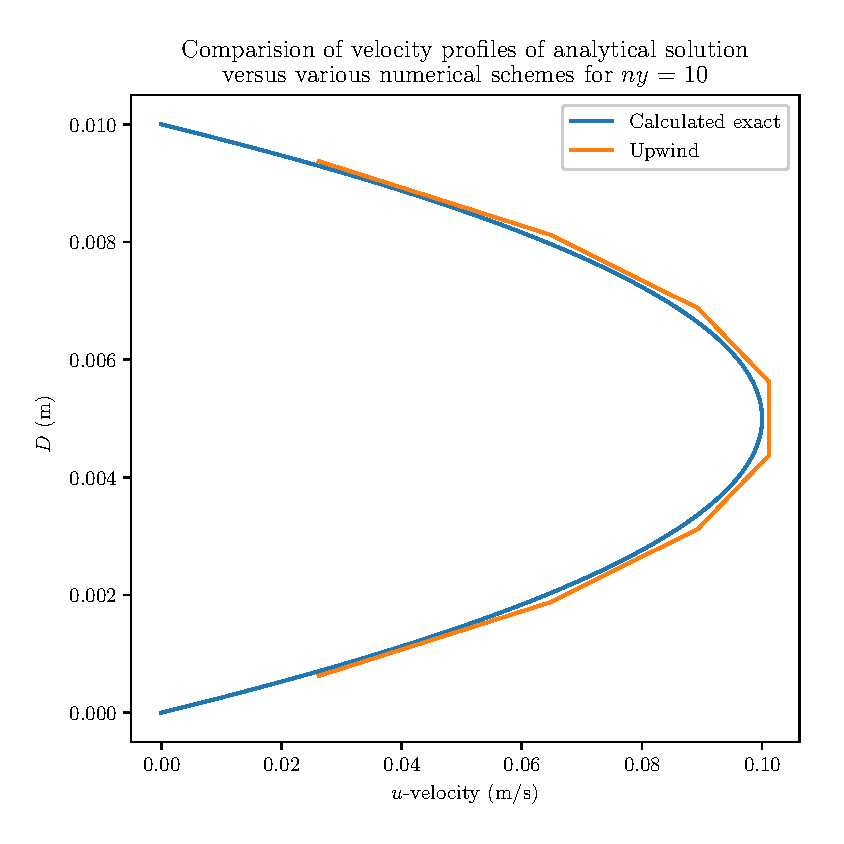
\includegraphics[width=0.5\textwidth]{ny-10_profilesComparison.eps}
    \caption{Results.}
    \label{fig:ny-10_profilesComparison.eps}
\end{figure}

\subsection{Future work}
\begin{itemize}
\item Remove the errors for 2D case
\item Modify the 3D code accordingly
\end{itemize}

\end{document}
